% Please do not change %
\documentclass[11pt]{article} % font size
\usepackage[margin=1in]{geometry} % margins
\usepackage{amsmath,amsthm,amssymb} % for the  common "math symbols"
\usepackage[shortlabels]{enumitem} % for enumeration
\usepackage{booktabs} % if you need tables
\usepackage{listings}
\usepackage{color}
\usepackage{tikzit}
\usepackage{tikzscale}
\usepackage{keycommand}
\usepackage{hyperref}
\usepackage{cite}
\usepackage{algorithm}
\usepackage{algpseudocode}
\usepackage{float}
\usepackage{listings}
\usepackage{xcolor}

% Define custom colors
\definecolor{lightgray}{gray}{0.95}
\definecolor{darkgreen}{rgb}{0.0, 0.5, 0.0} % Define darkgreen color here

\lstset{
    language=Python,
    basicstyle=\scriptsize\ttfamily,
    keywordstyle=\color{blue},
    commentstyle=\color{darkgreen},
    stringstyle=\color{red},
    showstringspaces=false,
    numbers=left,
    numberstyle=\tiny,
    frame=tb,
    backgroundcolor=\color{lightgray},
    breaklines=true, % Enable text wrapping
    columns=fullflexible, % Allow flexible column width
}

% \usetikzlibrary{circuits.ee.IEC}
\input{quantum.tikzstyles}
% \input{dots.tikzdefs}


\theoremstyle{definition}
\newtheorem{theorem}{Theorem}[section]
\newtheorem{corollary}[theorem]{Corollary}
\newtheorem{lemma}[theorem]{Lemma}
\newtheorem{proposition}[theorem]{Proposition}
\newtheorem{conjecture}[theorem]{Conjecture}
\newtheorem{definition}[theorem]{Definition}
\newtheorem{fact}[theorem]{Fact}

\renewcommand{\thesubsection}{\alph{subsection}}


% Feel free to include additional packages (if needed), but make sure it does not override the margin/font requirements.
%
\setlength{\parindent}{0pt} % no indent for new paragraphs.
\setlength{\parskip}{5pt} % distance between paragraphs, which will be used when you have a blank line in your LaTeX code.


%%%%%%%%%%%%%%%%%%%%%%%%%%%%%%%%%%%%%%%%%%%%%%%%%%%%%%%%%%%%%%%%%%%%%%%%%%%%%%
\title{Quantum Software Mini-Project}
%
\author{1081502}
\date{Hilary Term 2024}
%
\begin{document}


%
\maketitle

%You may use the usual \LaTeX\ environments to structure your answers:
%\begin{align}
%        \label{basegnn}
%        \mathbf{h}_u^{(t+1)} = \sigma \bigg( \mathbf{W}_\text{self}^{(t)} \mathbf{h}_u^{(t)}  + \mathbf{W}_\text{neigh}^{(t)} \sum_{v \in N(u)} \mathbf{h}_v^{(t)} + \mathbf{b}^{(t)} \bigg). 
%\end{align}


%\begin{table}[h]
%\caption{A simple table.}
%\centering
%\begin{tabular}[t]{lrrrr}
%\toprule
%Graphs & Can & Be  & Fun & Too \\ 
%\midrule 
%$G_1$ & $1$  & $2$ & $3$ & $4$ \\ 
%$G_2$ & $-1$  & $-2$ & $-3$ & $-4$ \\ 
%$G_3$ & $0.1$  & $0.2$ & $0.3$ & $0.4$ \\ 
%\bottomrule
%\end{tabular}
%\label{tab}
%\end{table}

\section{}
\subsection{}
The routine will decompose Clifford+T diagrams into a sum of classically computable stabiliser terms 
- 'Clifford' diagrams - building off of previous work \cite{sutcliffe2024procedurally, Kissinger_2022}.
Clifford+T diagrams can contain $T$-gates which make them more difficult to classically simulate, 
as opposed to Clifford, which are efficient to simulate classically.
Given $t$ $T$-gates ($T$-count), we can use identities found in previous work 
to obtain a sum of $2^{\alpha t}$ stabiliser terms.
The number of these terms is the dominant contributor to the efficiency of the decomposition.
The aim is to minimise the value of $\alpha$, and this work improves upon \cite{sutcliffe2024procedurally}.

\subsection{}
Previous work \cite{sutcliffe2024procedurally} uses a greedy approach to obtaining the best vertex cuts 
for efficient decomposition, based on a heuristic in the paper.
It also itself builds off the Brayvi, Smith, and Smolin (BSS) decomposition \cite{BSS2016} used 
and shown in PyZX \cite{kissinger2020Pyzx}.
This work improves the previous work by treating it as a search problem, 
and attempts to find a possibly more optimal cut based on the existing procedure.

In short, obtaining the heuristic can be described as follows \cite{sutcliffe2024procedurally}:
\begin{enumerate}
    \item Start at tier $t=0$.
    \item Assign weights at tier $t$ to CNOT vertices which separate $T$-like.
    CNOT vertices involved in separating separating less $T$-like spiders are given higher weights. 
    \label{step:assign}
    \item Proceed to the next tier $t \leftarrow t+1$, and similar to step \ref{step:assign},
    for any weighted previous tier vertex which is separated from fusing with lower tier weighted vertices,
    by CNOTs, add weights to the CNOT vertices.
    \item Repeat until no weightings are found at the largest tier $t=t_{max}$.
    \item Select among the vertices that has a positive weight in the highest tier, 
    the one whose maxmium across all tier is the largest. This will be the cut vertex.
\end{enumerate}
Some details are omitted for brevity.

The subsequent procedure (ProcCut) uses the heuristics to carry out simplification 
without compromising the graph structure and is described fully in \cite{sutcliffe2024procedurally}.

A key part of the procedure is using the following spider decomposition
to take advantage of the graph structure.

\begin{equation}
    \includegraphics{figures/spider_decomp_abs.tikz}
    \label{fig:spider_decomp}
\end{equation}

This work then makes use of the same heuristic and also considers other vertices among the highest tier to cut.
It uses Monte Carlo tree search (MCTS) to determine the strength of each vertex cut considered,
simulating the final $T$-count (MCTS ProcCut). 
MCTS has 4 main steps in each iteration \cite{chas2008}:
\begin{enumerate}
    \item Selection: From the root $R$, select child nodes which are more promising until a leaf node $L$
    \item Expansion: If $L$ is not terminal ($T$-count = 0), then expand the node and choose node $C$
    \item Simulation: Randomly playout from $C$ until we reach a terminal node
    \item Backpropogation: Use the result of the simluation to update nodes from $C$ to $R$.
\end{enumerate}
The MCTS setup is shown in Appendix \ref{app}.
In the case of Clifford+T diagram decomposition, 
a node can be described by a sum of graphs that need to be decomposed.
As a result, the final decomposition chosen will pick out the best sequence of decompositions that minimises
the final number of stabiliser terms and thus, effective $\alpha$.

This simple modification allows the algorithm to find cuts that are slight more optimal,
especially in the specific type of circuits used to benchmark \cite{sutcliffe2024procedurally}.

The algorithm below shows the function changed to obtain the list of possible vertices $v_{poss}$,
rather than the best vertex $v_{best} = \max_{w(v)} v_{poss}$, where $w(v)$ is the weight of vertex $v$.

\begin{algorithm}[H]
\caption{bestCut}
\label{alg:bestCutM}
\begin{algorithmic}[1]
\Require $g$: GraphS, $vweights_{max}$: list[int], $vtiers$: list[int]
\Ensure list of possible vertices
\State $maxTier \gets \max(vtiers)$
\State List of possible vertices $possV \gets []$
\For{$i$ in range($\text{len}(vweights_{max})$)}
    \State $w \gets vweights_{max}[i]$
    \If{$w \leq 0$ \textbf{or} $vtiers[i] \neq maxTier$}
        \State \textbf{continue}
    \EndIf
    \State $possV$.append($i$)
    \If{$g.phase(i) \in \{0.25,0.75,1.25,1.75\}$}
        \State $w \gets w + 1$ \Comment{Add 1 to weight if the prospective vertex to cut is itself T-like}
    \EndIf
\EndFor
\State \Return $possV$
\end{algorithmic}
\end{algorithm}


\subsection{}
Using the random circuit generation in \cite{sutcliffe2024procedurally},
we can benchmark in a similar manner.
MCTS ProcCut works well, especially if enough iterations of MCTS are allowed for leaf nodes to be explored.
It will always match or outperform the original algorithm.
The drawback, is of course, the complexity which is discussed in the last section.

Using the PyZX library \cite{kissinger2020Pyzx} function \texttt{zx.generate.cliffordT()}, 
we can also generate random circuits, varying the \texttt{qubit\_amount} and \texttt{gate\_count},
and making sure more $T$-gates and CNOT gates appear with 
\texttt{p\_t} and \texttt{p\_cnot}.
The details using this are described in the last section.

MCTS ProcCut working well for these circuits is to be expected 
as it is an extension of ProcCut \cite{sutcliffe2024procedurally} 
which takes advantage of the structure of $T$-gates being sandwiched between CNOT gates,
but simply considers more possible vertex cuts.

\subsection{}
The routine will always work since it falls back to BSS decomposition, similar to the original procedure.
However, it can be noted that it does have a limit of size and depth of circuit 
due to the exponential growth of both time and space,
that matches the previous work \cite{sutcliffe2024procedurally}.
The next section discusses the updated time and space complexity when using MCTS.

\subsection{}
As an example of where the routine would shine, below is an example of a ZX-diagram where the greedy heuristic
is not actually the optimal cut.
In the examples shown below, the graph of the left term obtained when using Equation \ref{fig:spider_decomp} 
is simplified using the ZX rewrite rules.

Here, the updated algorithm is able to immediately break decompose the graph in a single cut. 
Some steps are omitted for brevity - PyZX's \texttt{zx.simplify.full\_reduce()} was used to check the outcome.

\includegraphics[]{figures/initial.tikz}

$\to$ \raisebox{-0.5\totalheight}{\includegraphics{figures/cut_4.tikz}}

$\approx$ \raisebox{-0.5\totalheight}{\includegraphics[]{figures/cut_4_part.tikz}}
$\approx$ \raisebox{-0.5\totalheight}{\includegraphics[]{figures/cut_4_gh.tikz}}

$\approx$ \raisebox{-0.5\totalheight}{\includegraphics[]{figures/cut_4_mid.tikz}}
$\approx$ \raisebox{-0.5\totalheight}{\includegraphics[]{figures/cut_4_final.tikz}}
$\propto 1$


On the other hand, the original algorithm selects a suboptimal vertex cut.

\includegraphics[]{figures/initial.tikz}

$\to$ \raisebox{-0.5\totalheight}{\includegraphics[]{figures/cut_9.tikz}}

$\approx$ \raisebox{-0.5\totalheight}{\includegraphics[]{figures/cut_9_part.tikz}}
$\approx$ \raisebox{-0.5\totalheight}{\includegraphics[]{figures/cut_9_gh.tikz}}

$\approx$ \raisebox{-0.5\totalheight}{\includegraphics[]{figures/cut_9_final.tikz}}

We can analyse the actual performance of the algorithm 
using a similar benchmark as in \cite{sutcliffe2024procedurally}.
We then see that for the types of circuits described made of CNOTs, $\frac{n\pi}{4}$ phase gates, 
and Toffolis, when MCTS is able to explore leaf nodes, the number of stabiliser terms is reduced.

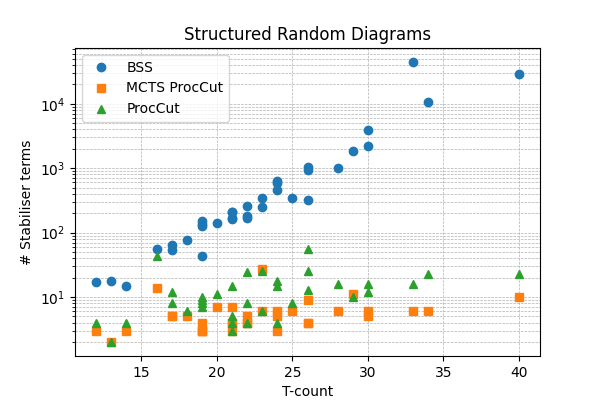
\includegraphics[width=0.5\textwidth]{figures/struct_stab.png}
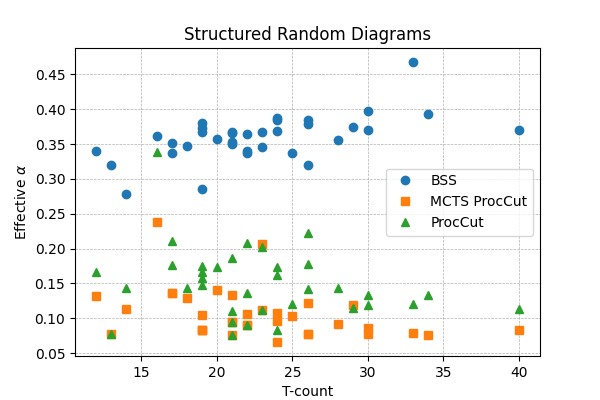
\includegraphics[width=0.5\textwidth]{figures/struct_alpha.png}

A good selection of the number of iterations for MCTS and number of children considered at each node
will allow for more optimal values of $\alpha$.
On the other hand, when MCTS is not able to complete due to not having enough iterations,
its performance can be unreliable.

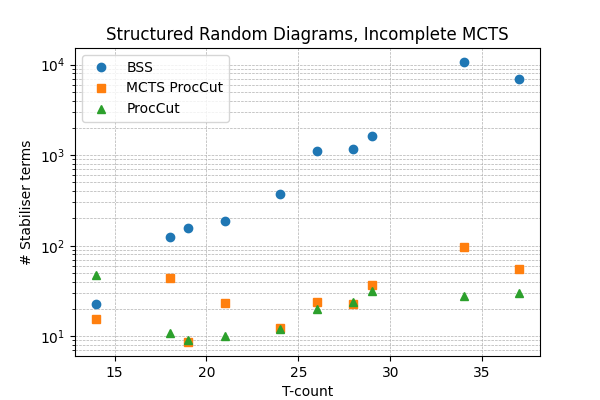
\includegraphics[width=0.5\textwidth]{figures/struct_inc_stab.png}
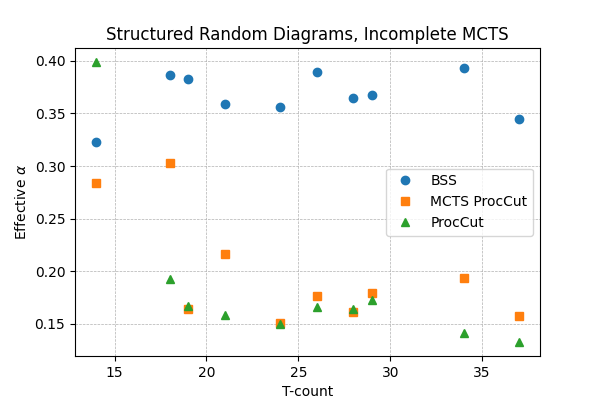
\includegraphics[width=0.5\textwidth]{figures/struct_inc_alpha.png}

The same algorithm was also tested using \texttt{zx.generate.cliffordT()} in PyZX,
where the benefit over BSS was not as clear as on the highly structured diagrams.
However, there are clear performance boosts over the original algorithm
if MCTS is able to complete exploring until the leaf nodes.
The configuration used, and their results are in the appendix \ref{app}.


Analysing the complexity, if the runtime of the original algorithm is $C$,
the MCTS makes it $O(Cvk)$, where $v$ is the number of random children,
and $k$ is the number of iterations.
Keeping $v$ low means that the change in runtime can be kept minimal 
while keeping the potential for finding the optimal cut.
Unless $P=NP$, we have that the $C$ will grow exponentially \cite{Bravyi2019simulationofquantum}, 
so no polynomial time solution is expected.
We find that the MCTS approach allows for flexibility between choosing a high number of iterations $k$,
versus a high number of random children $v$.
A high number of iterations will allow the algorithm to obtain the most optimal solution it can find,
since being able to explore until a leaf will mean it relies on BSS less, especially on the more structure diagrams.
A high number of random children will make it more likely it does not miss a more optimal solution.

Given the memory usage of the original algorithm to be $M$, 
the requirement to keep the search space grows with $O(Mv)$ with the current implementation.
This is a tradeoff, as it means it will run out of memory earlier than the original algorithm.

In conclusion, the addition of MCTS improves the base algorithm, 
with the tradeoff of having higher time and space complexity,
but allows for flexible configurations, and works very well with the more structured diagrams.

\clearpage
\appendix
\section{}
\label{app}

\begin{algorithm}
\caption{Monte Carlo Tree Search}
\label{alg:monte_carlo_tree_search}
\begin{algorithmic}[1]
\Require $root$: Node, $iterations$: int = 300
\For{$i$ in range($iterations$)}
    \State $leaf \gets$ selection($root$)
    \State $simulation\_result \gets$ simulation($leaf$)
    \State backpropagation($leaf$, $simulation\_result$)
\EndFor
\end{algorithmic}
\end{algorithm}

\lstinputlisting[language=Python]{node.py}

\texttt{zx.simplify.full\_reduce()} is used
with \texttt{qubit\_amount} varying from 6 to 8, and \texttt{gate\_count} varying from 50 to 150.
The probability of $T$-gates and CNOTs were chosen at \texttt{p\_t = 0.4} and \texttt{p\_cnot = 0.4}.

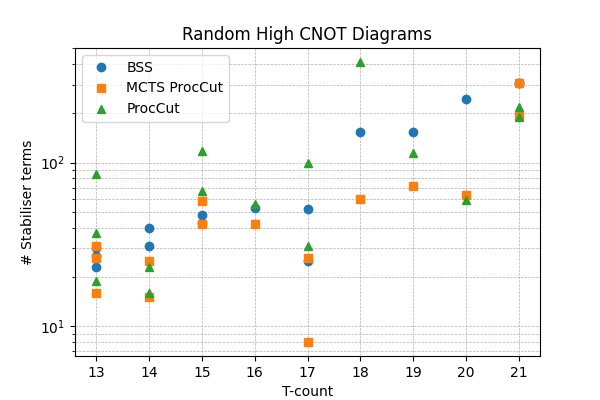
\includegraphics[width=0.5\textwidth]{figures/rand_stab.png}
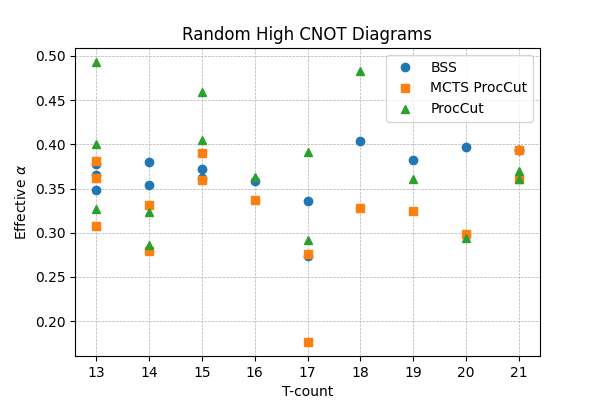
\includegraphics[width=0.5\textwidth]{figures/rand_alpha.png}

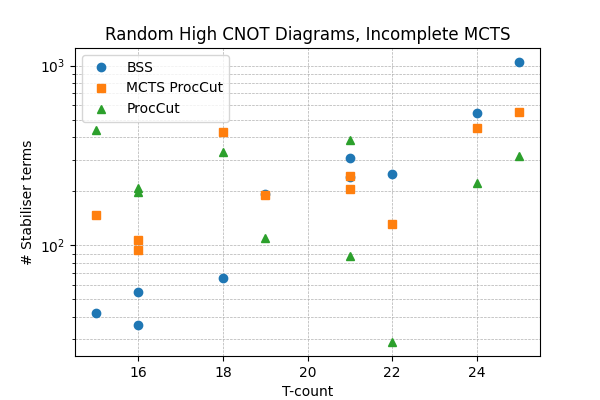
\includegraphics[width=0.5\textwidth]{figures/rand_inc_stab.png}
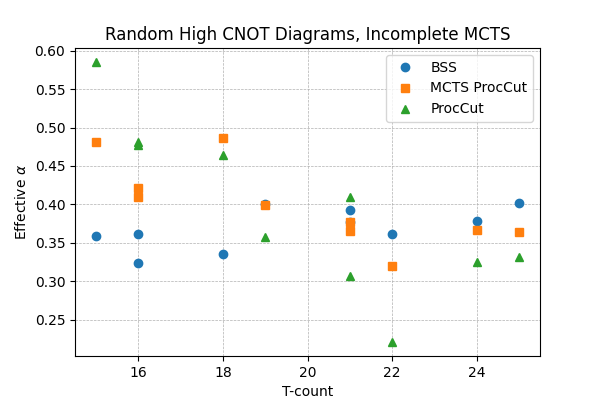
\includegraphics[width=0.5\textwidth]{figures/rand_inc_alpha.png}


\clearpage
\bibliographystyle{unsrt}
\bibliography{refs}

\end{document}